% Metódy inžinierskej práce

\documentclass[10pt,Slovak,a4paper]{article}

\usepackage[slovak]{babel}
%\usepackage[T1]{fontenc}
\usepackage[IL2]{fontenc} % lepšia sadzba písmena Ľ než v T1
\usepackage[utf8]{inputenc}
\usepackage{graphicx}
\usepackage{url} % príkaz \url na formátovanie URL
\usepackage{hyperref} % odkazy v texte budú aktívne (pri niektorých triedach dokumentov spôsobuje posun textu)

\usepackage{cite}
%\usepackage{times}

\pagestyle{headings}

\title{Porovnanie internetových prehladačov\thanks{Semestrálny projekt v predmete Metódy inžinierskej práce, ak. rok 2023/24, vedenie: Ing. Vladimír Mlynárovič PhD.}} % meno a priezvisko vyučujúceho na cvičeniach

\author{Tomáš Majerčík\\[2pt]
	{\small Slovenská technická univerzita v Bratislave}\\
	{\small Fakulta informatiky a informačných technológií}\\
	{\small \texttt{xmajercik@stuba.sk}}
}
	

\date{\small 5. November 2023} % upravte



\begin{document}



\maketitle

\begin{abstract}

V tejto práci sa zaoberáme porovnaním softvérov Chrome, Firefox, Edge a Brave. Pozrieme sa na ne nie len z hľadiska bezpečnosti, ale aj z pohľadu, ako tieto prehliadače zobrazujú a získavajú informácie. Zisťujeme, ktorý prehliadač najmenej zaťažuje hardvér (CPU (procesor) alebo RAM (operačná pamäť)), ktorý je najpopulárnejší, najdostupnejší a najobľúbenejší medzi používateľmi, ktorý ponúka najlepšie prostredie a prostriedky pre vývoj webových aplikácií a samozrejme aj pohľad na poskytnutú bezpečnosť či súkromie. V článku sa snažíme na základe získaných informácií o porovnanie výhod a nevýhod daných prehliadačov. Výsledky tejto práce môžu slúžiť ako prostriedok pre čitateľov pri vyberaní ich nového obľúbeného softvéru.


\end{abstract}



\section{Úvod}
%uvod
    \begin{paragraph}
        Technologický rozvoj dneštnej doby nás doviedol k neuveriteľne veľkému rozmachu internetu. V dnešnej dobe je internet neoddeliteľnou súčasťou nášho života. Využívame ho každý deň pri bežnej práci, štúdiu, či zábave alebo oddychu. Aby sme mohli naplno využívať potenciál internetu, potrebujeme dobrý internetový prehliadač. \\ \\
        Internetové prehliadače sú jednou z najdôležitejších súčastí nášho každodenného života. Internetové prehliadače sú softvérové aplikácie, ktoré nám umožnujú pohodlne, ako aj názov napovedá, prehliadať internet. Existuje mnoho rôznych prehliadačov, pričom sú všetky dennodenne vyvíjané a vylepšované tak, aby čo najlepšie uspokojili svojích koncových uživateľov. Každý z nich má však svoje silné a slabé stránky. \\ \\
        V tomto článku sa pozrieme na aktuálne obľúbené prehliadače na trhu. Budeme sa zaoberať ich základnými vlastnosťami, ako je bezpečnosť, zaťaženie systému alebo kompatibilita. Okrem toho sa pozrieme aj na ich špeciálne funkcie, ako je podpora rozšírení, blokovanie reklám či ochrana súkromia.
    \end{paragraph}

    
    \subsection{Princípy internetových prehliadačov}
    \begin{paragraph}
        Hlavnou funkciou internetových prehliadačov je zobraziť uživateľom vybraný obsah tak, že ho vyžiada zo serveru a zobrazí sa v rozhraní prehliadača. Obsah je zvyčajne HTML dokument, PDF dokument alebo obrázok či iné. Moderné internetové prehliadače zvyčajne zdieľajú podobné prvky uživateľského rozhrania. 
        
        \begin{enumerate}
          \item Otvorené karty
          \item Riadok na vloženie/zobrazenie URL adresy
          \item Tlačidlá "späť" a "dopredu"
          \item Tlačidlo na reload [znovu načítanie] stránky a tlačidlo na zastavenie načitávania
          \item možnosti záložiek
          \item Rozšírenia, nastavenia a ďalšie
        \end{enumerate}

        \subsubsection{Vykresľovanie webových stránok}
        Vykresľovanie webových stránok je proces, pri ktorom sa dáta stránky zobrazujú na obrazovke počítača. Tento proces sa skladá z troch hlavných krokov:
        \begin{enumerate}
            \item Parsing: je to proces rozdelenia HTML dokumentu na strom uzlom pričom každý uzol predstavuje jeden element v dokumente
            \item Renderovací strom: je strom uzlov, ktoré predstavujú vizuálne prvky webovej stránky
            \item Vykreslenie renderovacieho stromu: vykresľovacia jednotka vykresľuje renderovací strom na obrazovku tak, že každému prvku presne pridelí súradnicu pixelov kde sa na obrazovke majú zobraziť
        \end{enumerate}
        
        %obrazok
        \begin{center}
            
\includegraphics[scale=.8]{uvod.png}
            \cite{img1}
        \end{center}
        
        \subsubsection{Rendering engines[software pre vykresľovanie]}
            Rôzne prehliadače používajú rozličné software pre vykresľovanie. Internet Explorer používa Trident, Firefox Gecko, Safari používa WebKit. Chrome and Opera zasa Blink, ktorý bol vyvinutý na zaklade WebKit-u. 
            Sofrware pre vykresľovanie je zodpovedný za konvertovanie HTML, JavaScript a CSS do vizuálnej podoby. Tento software zastrešuje proces spomenutý v odseku 1.1.1.
            WebKit, ako aj Gecko či Trident sú velmi výkonné engine-y ktoré dokážu vykresľovať komplexné webové aplikácie s ľahkosťou. Sú navrnhnuté tak, aby boli čo najefektívnejšie čo ma za následok rýchle načitavanie stránok.\\
            \cite{ako_prehliadace_funguju}
            \pagebreak
    \end{paragraph}    
%uvod 
\section{Jadro}
%jadro
    \subsection{Hardwarové zaťaženie}
    \begin{paragraph}
    
        \textbf{Porovnanie rozličných prehliadačov v mnohých testoch na     základe ktorých vyhlásime najlepší prehliadač v danej sekcii}. \\\\
            V tomto teste bol použitý počítač s 16GB RAM, i7 Intel CPU, 500GB SSD a 64bit-ový windows 11 
            \subsubsection{CPU (zaťaženie procesora)}
            Test bol prevedený použitím aplikácie Speedometer. Speedometer je test ktorý spustí 200 web stránok pričom pri návšteve každej stránky spočíta čas ktorý bol potrebný na načítanie stránky. Týmto je vyhodnotené zaťaženie procesora jednotlivými priehľadačmi.
        \begin{figure}[h]
            \centering
            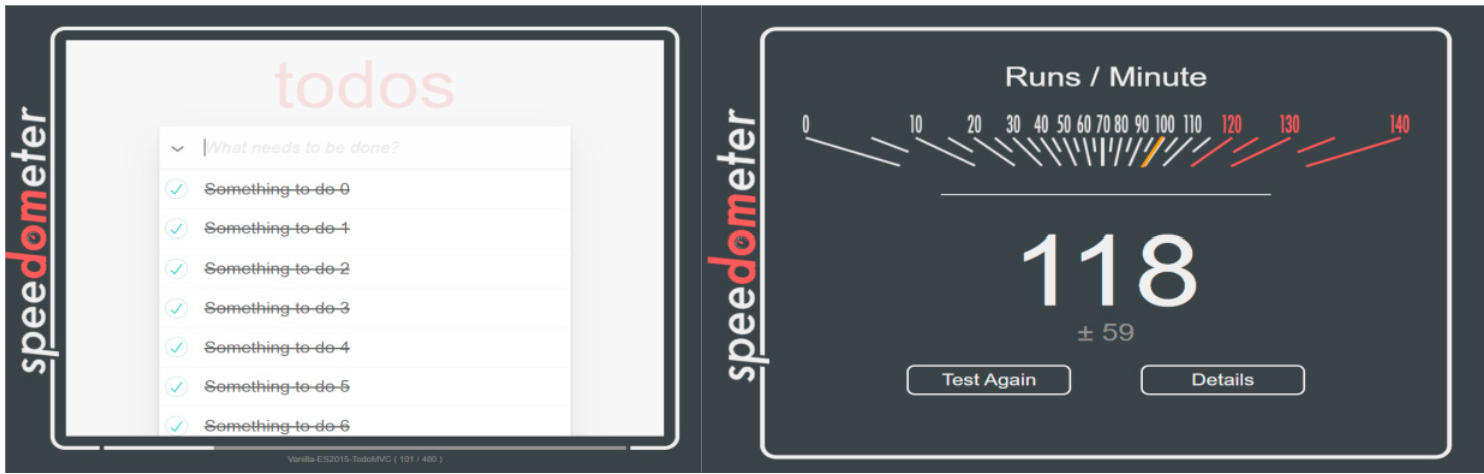
\includegraphics[scale=.60]{speedometer.png}
            \cite{img2}
            \caption{test prehliadačov (naľavo) a výledky (napravo)}
            \label{fig1}
        \end{figure}    
        
        Obrázky \ref{fig1} ukazujú ako Speedometer testuje prehliadače. Speedometer spočíta počet kariet kroré boli úspešne otvorené / načítané. \\

        \begin{figure}[h]
            \centering
            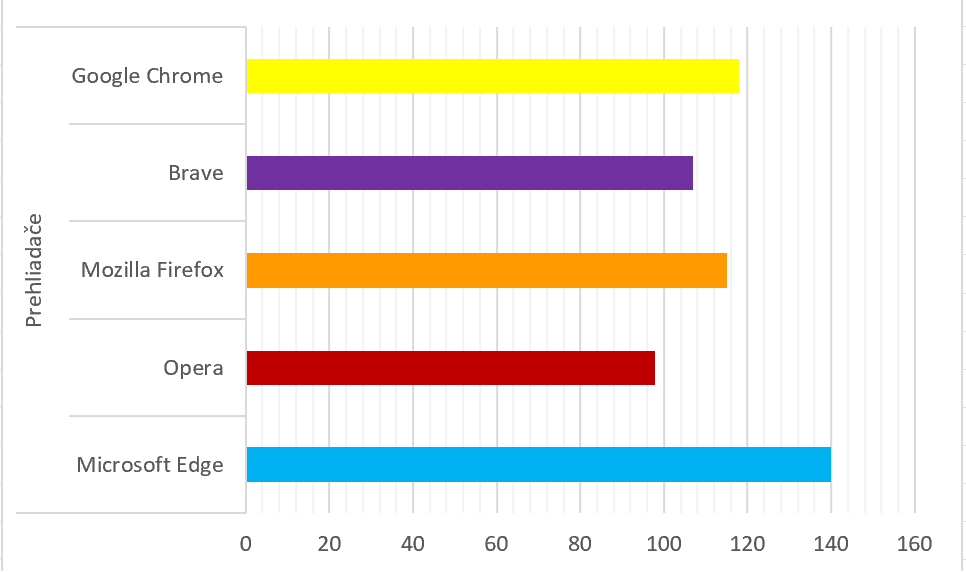
\includegraphics[scale=.8]{graph1.png}
            \cite{graph1}
            \caption{výsledky testovania jednotlivých prehliadačov}
            \label{graph1}
        \end{figure}   

        Obrázok \ref{graph1} znázorňuje výsledky testu. Musíme však mať na pamäti, že jednotlivé prehliadače nemusia byť pre daný test optimalizované. Napriek tomu však môžme povedať, že \textbf{ Microsoft Edge} zatiaľ vedie a najhoršie dopadla \textbf{Opera}.
        \cite{browser_comparison}
    \end{paragraph}

        
    \subsubsection{RAM (zaberanie operačnej pamäte)}
    \begin{paragraph}
        Test bol prevedený takto: V danom prehliadači bolo otvorených 10 kariet, každá inej kategórie, kde následne bolo zmerané koľko pamäte prehliadač využíva.

        \begin{figure}[h]
            \centering
            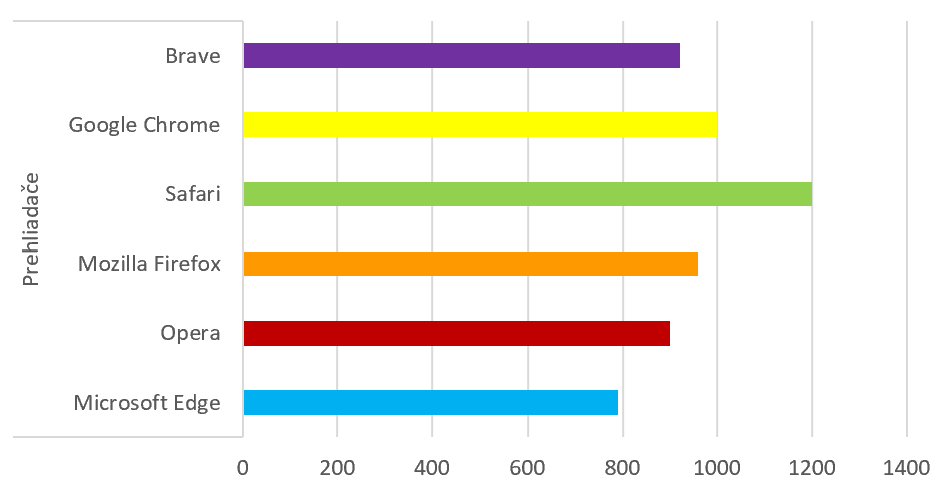
\includegraphics[scale=.7]{graph2.png}
            \cite{graph2}
            \caption{výsledky testovania jednotlivých prehliadačov (udané v MB)}
            \label{graph2}
        \end{figure}  
        
        Obrázok \ref{graph2} zobrazuje porovnanie, koľko pamäte prehliadač využíval. Google Chrome potreboval 1000 MB dát, Brave 920 MB, Mozilla Firefox použila 960 MB, , Opera 899 MB, Apple Safari 1200 MB a Microsoft Edge 790 MB čo ho robí najlepším aj v tejto kategórii. Naopak Apple Safari potreboval najväčšie množstvo pamäte.
        \cite{browser_compare_ram}

        %Na pevnom disku tieto prehliadače zaberajú následne:

        \begin{itemize}
          \item Google Chrome: 153.91 MB
          \item Safari: 1.68 MB
          \item Mozilla Firefox: 40 MB
          \item Opera: 3.5 MB
          \item Microsoft Edge: 112 MB
          \item Brave: 200 MB
        \end{itemize}

        \begin{picture}(0,0)
          \put(100,-120){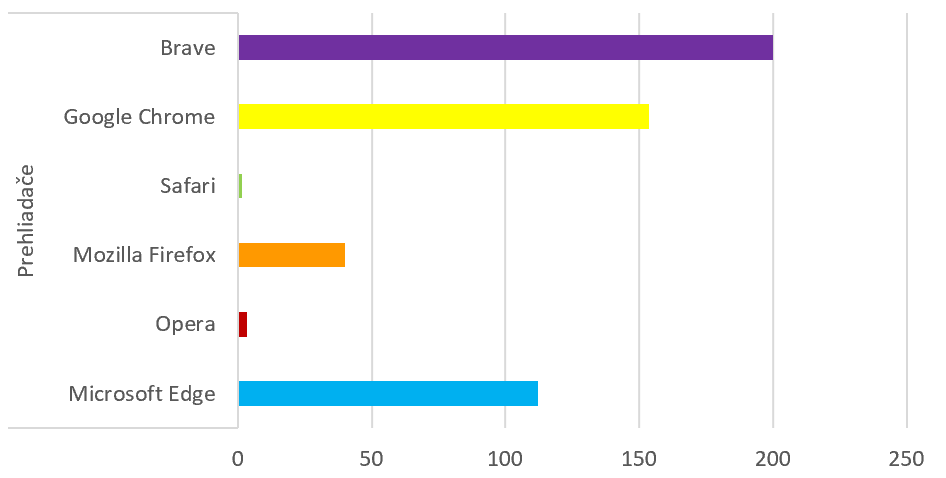
\includegraphics[scale=.8]{graph3.png}}
        \end{picture}

        \pagebreak
    \end{paragraph}

    \subsubsection{GPU (grafická náročnosť)}
    \begin{paragraph}
    Graficku náročnosť prehliadačov budeme testovať pomocou MotionMark testeru. MotionMark je test pre prehliadače zameraný na grafický výkon prehliadačov. Test funguje tak, že na obrazovku vykresľuje veľké množstvo grafických elementov za pomoci HTML, CSS a JavaScript-u. Na základe zistených dát MotionMark vyhodnotí dosiahnuté skóre. 

    \begin{figure}[h]
        \centering
        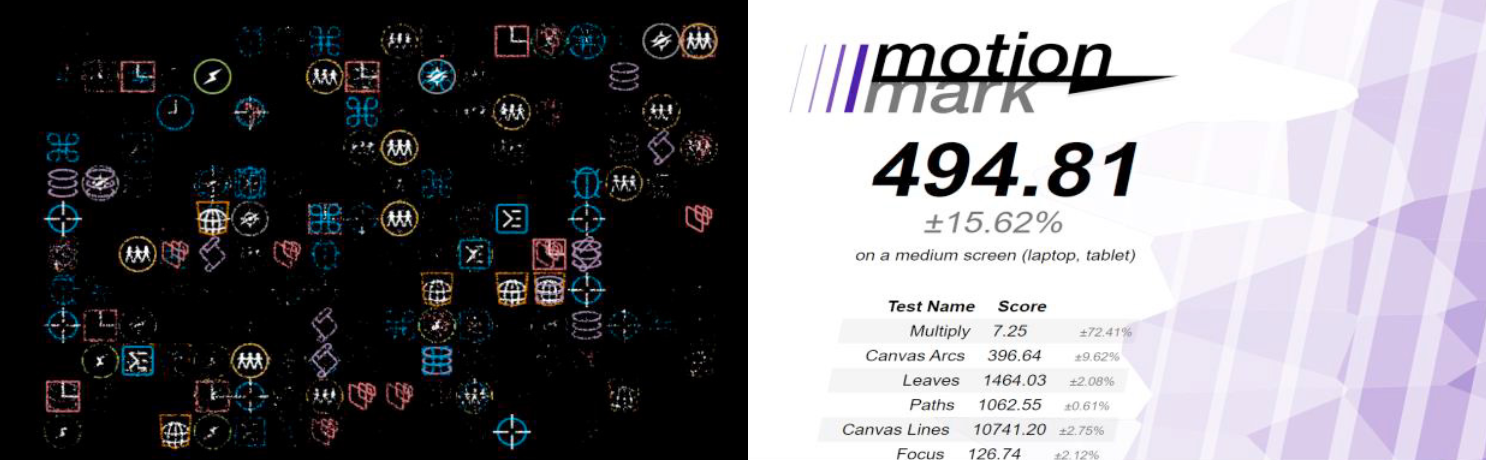
\includegraphics[scale=.7]{motionmark.png}
        \cite{img3}
        \caption{MotionMark test (naľavo), výsledky (napravo)}
        \label{img3}
    \end{figure} 

    Obrázky \ref{img3} ukazujú ako MotionMark testuje prehliadače.\\

    \begin{figure}[h]
        \centering
        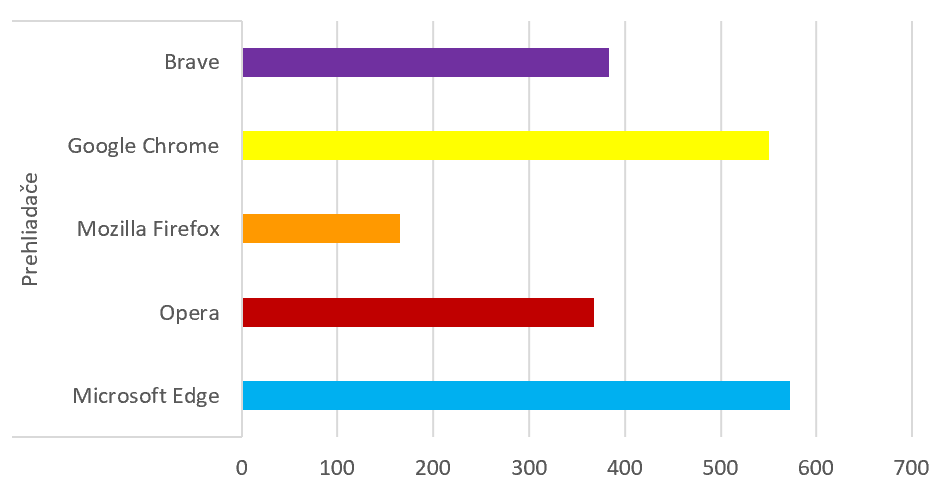
\includegraphics[scale=.8]{graph4.png}
        \cite{graph4}
        \caption{výsledky testovania jednotlivých prehliadačov (udané v MB)}
        \label{graph4}
    \end{figure}  

    
        \cite{browser_comparison}
    \end{paragraph}

    \subsubsection{Zhodnotenie}
    \begin{paragraph}
        Nie je jednoduché určiť priameho výťaza v týchto testoch. Microsoft Edge dobre používa a zbytočne nezaťažuje CPU a RAM ale zasa viac zaťažuje GPU kdežto napríklad Chrome dobre využíva GPU no zahltí väčšie množstvo RAM a CPU. Dobrým kompromisom môže byť Mozilla Firefox keďže je takmer vo všetkom zlatou strednou cestou.
        \pagebreak
    \end{paragraph}
        

        
    \subsection{Zabezpečenie a súkromie prehliadačov}
        Bezpečnosť a súkromie prehliadačov je neustále aktuálnou a často diskutovanou témou. Prehliadače nám umožnujú pristupovať k enormnému počtu informácii a umožňujú vykonávať veľa online činností. Spolu s narastaním počtu informácií narastá aj záujem o našu osobnú bezpečnosť a pocit súkromia. Spoliehame sa na prehliadače, že nás ochránia. \\
        V dneštnej dobe existuje mnoho nástrah a rizík ktoré môžu postihnúť internetových uživateľov. Akonáhle je zariadanie pripojené k intenetu, môžeme si byť istý, že musí odolávať útokom. Spoliehame sa však na prehliadače, ktoré nás majú ochrnániť. Ako to však je? Sú naozaj bezpečné a dokážu dobre šifrovať dáta?

        \begin{paragraph}
            Prehliadače nefungujú samostatne, ale fungujú v spojení s backendovou infraštruktúrou. Väčšina prehliadačov využíva služby bezpečného prehliadania na
            chránenie používateľov pred phishingovými a malvérovými stránkami. Prehliadače tiež kontaktujú backendové servery, aby kontrolovali aktualizácie. 
            \cite{cite_whattheydo} \\
            Medzi najčastejšie nebezpečie patria phishingové útoky
        \end{paragraph}
        \subsubsection{Detekcia phishing útokov}
            \begin{paragraph}
                Ako uvádzajú Noman Mazher, Imran Ashraf a Ayesha Altaf, "Phishing is the technique of social engineering in which important information of user such as credit card, email password etc are hijacked" \cite{6732784}. \\ Phishing je forma útoku kde sa útočník vydáva za dôveryhodný a spoľahlivý zdroj snažiaci sa vylákať citlivé informácie od svojích obetí. Medzi typické phishingové útoky patrí metóda, keď útočík rozošle falošný e-mail ktorý sa tvári ako dôveryhodná listina napr. z Bankovej spoločnosti vyzývajúca obete aby sa prihlásili na falošnú web stránku odkiaľ sú následne nešifrované údaje poskytnuté útočnikovi.
            \end{paragraph}
            \begin{paragraph}
                Najjednoduchší spôsob ako môže prehliadač ochrániť uživateľov pred phishing útokmi je pridanie URL adries odhalených phishingových stránok na čiernu listinu a tak ich zablokovať aby sa ku ním uživatelia nemohli dostať. \\
                Toto však nie vždy funguje keďže dennodenne vznikajú nové stránky ktoré nie sú na čiernej listine. Ďalšia metóda sa nazýva heuristic-based approach [zo starovekého Gréckeho slova heurískō 'nájsť, objaviť']. Toto sa snaží odhaliť podvodné stránky na základe obsahu stránky. Boli predstavené systémy na základe umelej inteligencie na detekciu podvodných stránok. Dalšou metódov je použitie bezpečnostných nástrojov.
            \end{paragraph}


        
    \subsection{Popularita jednotlivých prehliadačov}
        yes, it's chrome
    \subsection{Porovnanie prostredí pre vývoj}
        you guessed it, edge is not the one




%jadro
\section{Záver} \label{zaver} % prípadne iný variant názvu





%\cite{literature}

%\acknowledgement{Ak niekomu chcete poďakovať\ldots}


% týmto sa generuje zoznam literatúry z obsahu súboru literatura.bib podľa toho, na čo sa v článku odkazujete
\pagebreak
\bibliography{literatura.bib}
\bibliographystyle{abbrv} % prípadne alpha, abbrv alebo hociktorý iný
\end{document}
